\section{Results}
\label{sec:results}

\todo{This is the results section}

We present a comparison between the usage characteristics of the control\footnote{gateway byte counters from users with a 105 Mbps access link} and test\footnote{gateway byte counters from users with a 105 Mbps access link}. We interpret the results as change in usage behavior due to increase in access link bandwidth. %although these are two separate sets of devices we interpret them as changes as explained in "methodology" or "data"

\subsection{User Behavior}
\label{subsec:behavior}

\hypoth{1}. Does aggregate user behavior differ?

%%%%%%%%%%%%%%%%%%%%%%%%%%%%%%%%%%%%%%%%%%%%%%%%%%%%%%%%%%%%%%%%%%%%%
\begin{figure}[t!]
%\hspace*{-0.2in}
\begin{minipage}{1\linewidth}
\centering
%
%\hfill
\begin{subfigure}[b]{\linewidth}
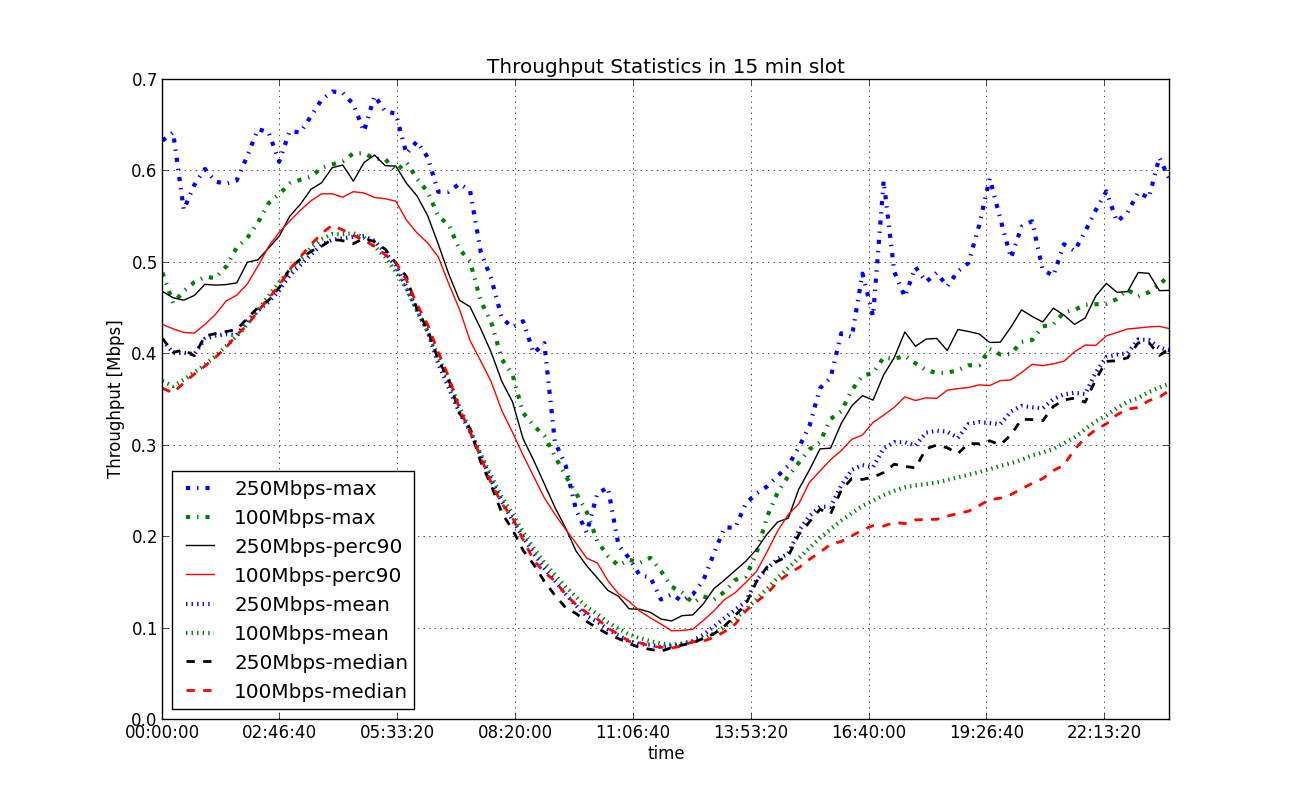
\includegraphics[width=\linewidth]{figures/describe-total-throughput-per-day[replace].png}
  \caption{agg (days) over means (devices)}
  %http://riverside.noise.gatech.edu:8083/separated/full/describe-total-throughput-per-day.png
  \label{fig:TS-data-rate-daily}
\end{subfigure}
%
\vspace{-1em}
%
\begin{subfigure}[b]{\linewidth}
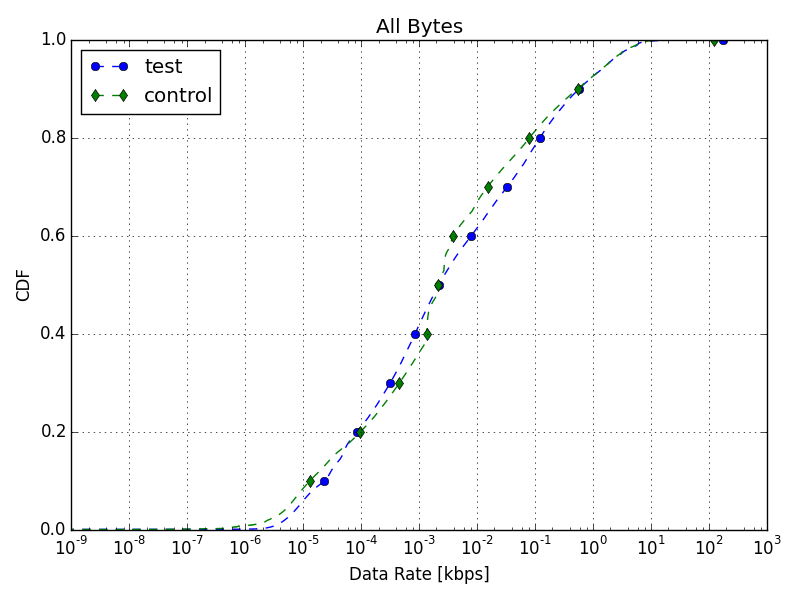
\includegraphics[width=\linewidth]{figures/cdf-all-bytes.png}
  \caption{CDF of data rate per time slot for all devices (agg view of data)}
  \vspace{1em}
  %http://sites.noise.gatech.edu/~sarthak/files/comcast/plots/full_dw/cdf-all-bytes.png
  \label{fig:CDF-data-rate-all}
\end{subfigure}
%\hfill
\end{minipage}
\caption{User Behavior: Overall not much change due to capacity increase}
\label{fig:user-behavior}
% created using docs/metadata-separated.log
\end{figure}
%%%%%%%%%%%%%%%%%%%%%%%%%%%%%%%%%%%%%%%%%%%%%%%%%%%%%%%%%%%%%%%%%%%%%

no dip pattern

usage is similar 


\subsection{Peak Utilization}
\label{subsec:peak-util}

\hypoth{2}. Does the maximum (or 90-\%ile) data transferred by the device differ?


%%%%%%%%%%%%%%%%%%%%%%%%%%%%%%%%%%%%%%%%%%%%%%%%%%%%%%%%%%%%%%%%%%%%%
\begin{figure}[t!]
%\hspace*{-0.2in}
\begin{minipage}{1\linewidth}
\centering
%
%\hfill
\begin{subfigure}[b]{\linewidth}
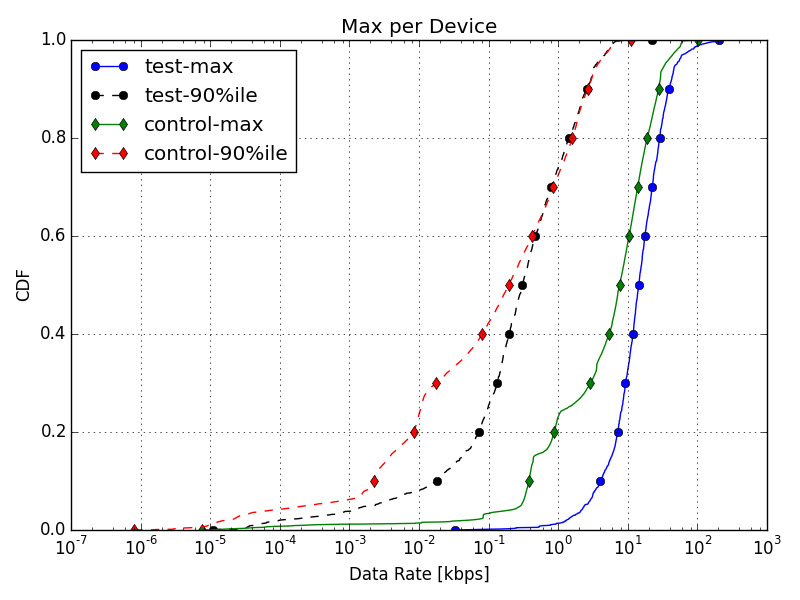
\includegraphics[width=\linewidth]{figures/cdf-max-per-device.png}
  \caption{CDF of max per device}
  %http://sites.noise.gatech.edu/~sarthak/files/comcast/plots/full_dw/cdf-max-per-device.png
  \label{fig:CDF-data-rate-max}
\end{subfigure}
%
\vspace{-1em}
%
\begin{subfigure}[b]{\linewidth}
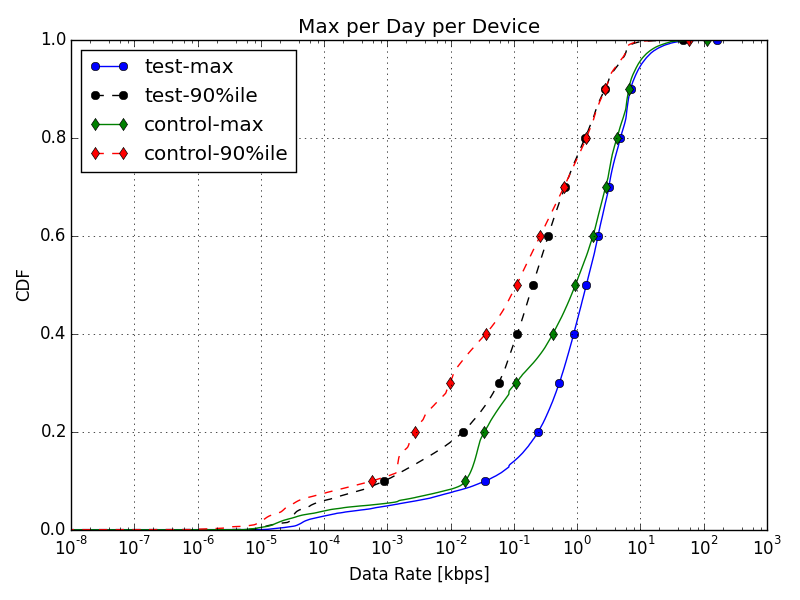
\includegraphics[width=\linewidth]{figures/cdf-max-per-day-per-device.png}
  \caption{CDF of max per device daily}
  \vspace{1em}
  %http://sites.noise.gatech.edu/~sarthak/files/comcast/plots/full_dw/cdf-max-per-day-per-device.png
  \label{fig:CDF-data-rate-max-daily}
\end{subfigure}
%\hfill
\end{minipage}
\caption{Peak Utilization: The maximum data rate varies for test and control set for low data rates, and this variation is present daily.}
\label{fig:peak-utilization}
% created using docs/metadata-separated.log
\end{figure}
%%%%%%%%%%%%%%%%%%%%%%%%%%%%%%%%%%%%%%%%%%%%%%%%%%%%%%%%%%%%%%%%%%%%%

copy reasons from ppt



\subsection{Prime Time Ratio}
\label{subsec:prime-time}

\hypoth{3}. Does the prime-time ratio differ?

Measure PT = avg data rate during a peak hour period : off-peak period

updated to 8-12 PM as seen from ~\ref{fig:TS-data-rate-daily}.

\sg{can also include PT table from ppt if worth it -- table shows the "no dip" pattern similar to time series in first subsection.}


%%%%%%%%%%%%%%%%%%%%%%%%%%%%%%%%%%%%%%%%%%%%%%%%%%%%%%%%%%%%%%%%%%%%%

\begin{figure}[t!]
\begin{minipage}{1\linewidth}
\centering
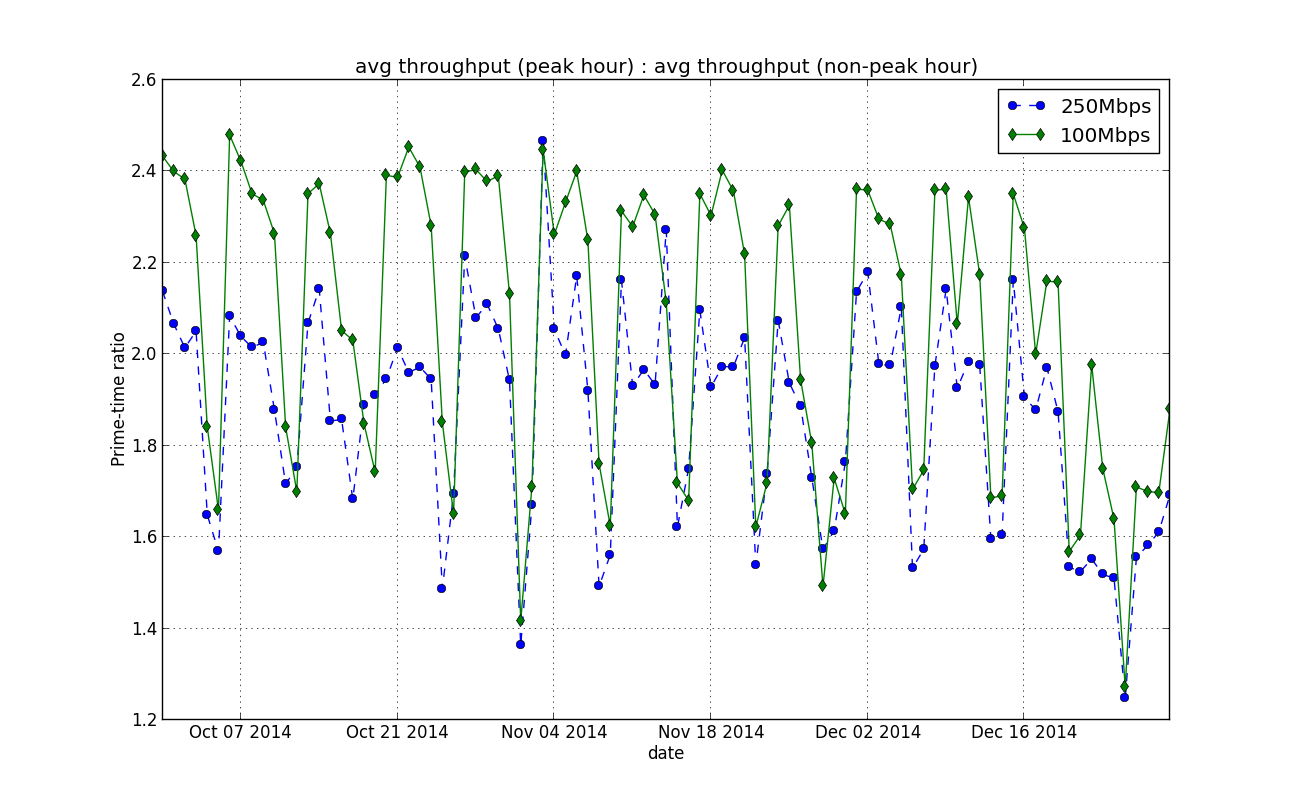
\includegraphics[width=\linewidth]{figures/prime-time-ratio-by-date[replace].png}
\caption{Prime Time ratio showing weekly pattern + differences during holiday periods (Thanksgiving, Christmas)}
%http://riverside.noise.gatech.edu:8083/separated/full/prime-time-ratio-by-date.png
\label{fig:TS-prime-time-ratio}
\end{minipage}
\end{figure}

%%%%%%%%%%%%%%%%%%%%%%%%%%%%%%%%%%%%%%%%%%%%%%%%%%%%%%%%%%%%%%%%%%%%%



% \sg{ http://riverside.noise.gatech.edu:8083/separated/full/cdf-prime-time-ratio-per-device.png not needed ? }

\subsection{Peak Ratio}
\label{subsec:peak-ratio}

\hypoth{4}. How much does the traffic vary in a single day?

%%%%%%%%%%%%%%%%%%%%%%%%%%%%%%%%%%%%%%%%%%%%%%%%%%%%%%%%%%%%%%%%%%%%%

\begin{figure}[t!]
\begin{minipage}{1\linewidth}
\centering
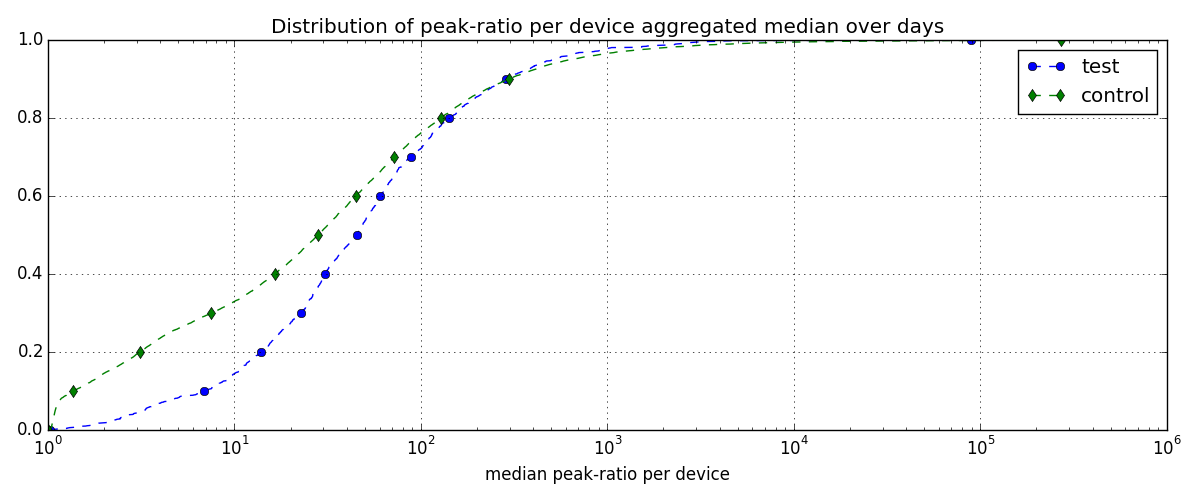
\includegraphics[width=\linewidth]{figures/peakratio-CDF-devices-MEDIAN.png}
\caption{Median peak ratio per device showing that test set has higher daily variance, which goes upto 50 times)}
%http://sites.noise.gatech.edu/~sarthak/files/comcast/plots/full_dw/peakratio-CDF-devices-MEDIAN.png
\label{fig:CDF-peak-ratio-median}
\end{minipage}
\end{figure}

implies that ISPs should condition their networks to 50 times median usage per user

%%%%%%%%%%%%%%%%%%%%%%%%%%%%%%%%%%%%%%%%%%%%%%%%%%%%%%%%%%%%%%%%%%%%%


%
%big difference (2 x median ratio) in per device per day ratios of 90%ile:median.
%weird shape again for values < ratio 100
%big difference in this ratio per day, and it is consistent across all individual sets + months.
%very large for Dec, slightly smaller for Nov
%interestingly, at higher ratios control is slightly > test. This means that certain devices in control set have a huge std (ratio) in a day as compared to test set which has a lower “max” ratio.
%


\subsection{Traffic Asymmetry}
\label{subsec:asymmetry}
\todo{maybe this doesn't need a separate section, just comment on asymmetry in each of the above - plot uplink also}
